\documentclass[unknownkeysallowed]{beamer}

\usepackage[utf8]{inputenc}
\usepackage{graphicx}
\usepackage{epsfig}
\usepackage{hyperref}
\usepackage{booktabs, caption}
\usepackage{color}
\usepackage{tikz}


\beamertemplatenavigationsymbolsempty

\mode<presentation>
{
  \usetheme{sebslides}
  \setbeamertemplate{items}[circle]
}

\definecolor{uipoppy}{RGB}{225, 64, 5}
\definecolor{tumblue}{RGB}{0,100,188}
\definecolor{uipaleblue}{RGB}{96,123,139}
\definecolor{uiblack}{RGB}{0, 0, 0}

\newcommand{\topline}{%
  \tikz[remember picture,overlay] {%
    \draw[line width=0.35mm, uipaleblue]
    ([yshift=-1.2cm]current page.north west)
    -- ([yshift=-1.2cm,xshift=\paperwidth]current page.north west);}}

\title{Data Mining with Spare Grids}
\subtitle{Seminar: Computational Aspects of Machine Learning}
\author{Sebastian Kreisel}
\date{\today}

\begin{document}

{
\setbeamertemplate{footline}{}
\begin{frame}
  \maketitle
  \vspace{15px}
  \begin{center}
    \color{tumblue}{\footnotesize{Technische Universität München}}\\
    \vspace{6px}
    \includegraphics[width=1cm]{tum}
  \end{center}
\end{frame}
}
\addtocounter{framenumber}{-1}

\begin{frame}
  \frametitle{Overview}
  \topline
  \vspace{-10px}
  \begin{itemize}
    \item Motivation for Sparse Grids
      \vspace{8px}
    \item Sparse Grids: Basics
      \vspace{8px}
    \item Sparse Grids: Machine Learning
      \vspace{8px}
    \item Examples with Data Sets
      \vspace{8px}
    \item Parallelization and Implementation
  \end{itemize}
\end{frame}

\begin{frame}
  \frametitle{Motivation for Sparse Grids}
  \topline
  \vspace{-10px}
  \begin{block}{Grid based approaches in ML}
    \begin{itemize}
      \item Discretizes the space into a grid
      \item Basis--functions around grid points, not data points
    \end{itemize}

    \begin{figure}[!htb]
      \setbeamertemplate{caption}{\raggedright\insertcaption\par}
      \setbeamerfont{caption}{size=\footnotesize}
      \minipage{0.45\textwidth}
      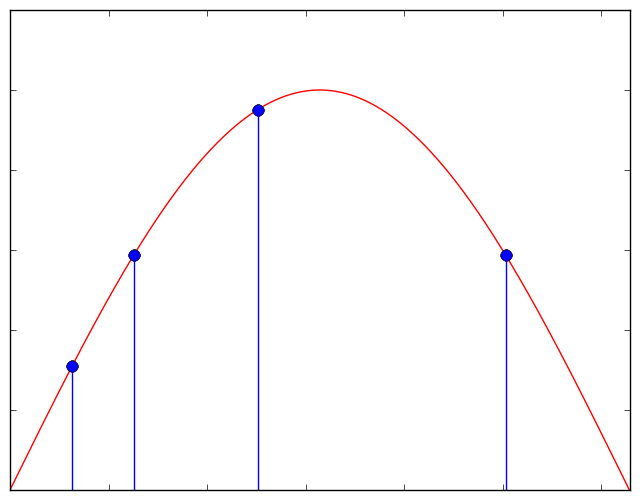
\includegraphics[width=\linewidth]{images/pointbase.png}
      \vspace{-12px}
      \caption{Point based}
      \endminipage
      \hspace{0.025\textwidth}
      \minipage{0.45\textwidth}
      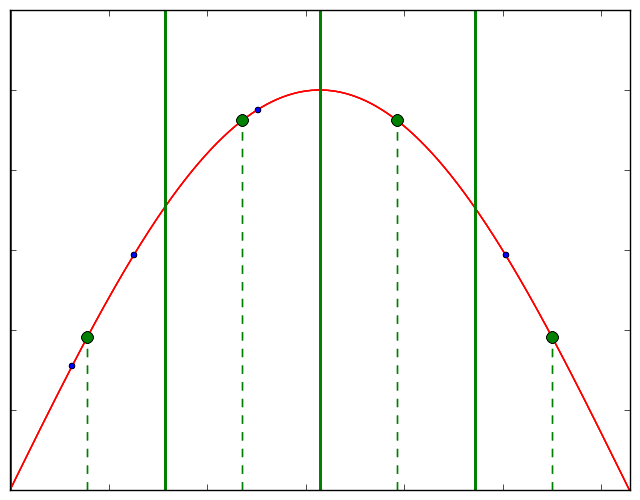
\includegraphics[width=\linewidth]{images/gridbase.png}
      \vspace{-12px}
      \caption{Grid based}
      \endminipage
    \end{figure}
  \end{block}
\end{frame}

\begin{frame}
  \frametitle{Motivation for Sparse Grids}
  \topline
  \vspace{-10px}
  \begin{block}{Suitable for}
    \begin{itemize}
      \item Big datasets
      \item Easily/automatically classifiable data
      \item Medical, seismic, commercial data
    \end{itemize}
  \end{block}
  \begin{block}{Curse of dimensionality}
    \begin{itemize}
    \item The volume of a space is exponential in it's dimensions
    \item The amount of training data required becomes unmanageable
      \begin{itemize}
      \item because of lacking computational/storage capacities
      \item because data acquisition is expensive
      \end{itemize}
    \item Becomes relevant for $d > 3$
    \item \textbf{Applies to full-grid discretization}
    \end{itemize}
  \end{block}
\end{frame}

%%% Local Variables:
%%% TeX-master: "slides"
%%% End:
\begin{frame}
  \frametitle{Full Grid Discretization}
  \topline1
  \vspace{-10px}
  \begin{block}{1. Function to discretize}
    \begin{figure}[!htp]

      \setbeamertemplate{caption}{\raggedright\insertcaption\par}
      \setbeamerfont{caption}{size=\footnotesize}
      \centering
      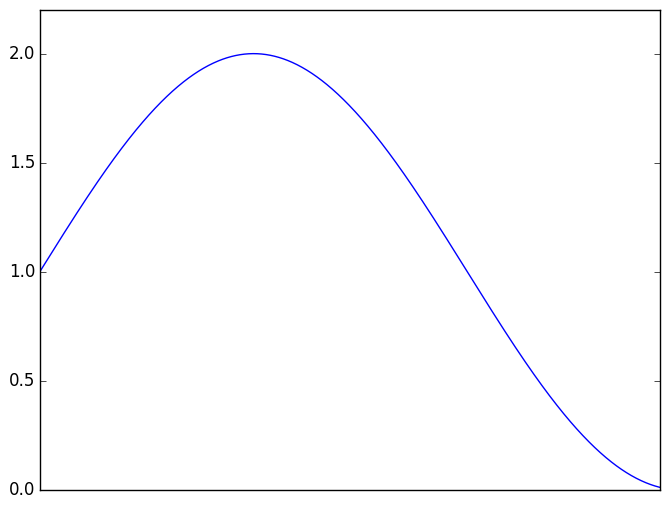
\includegraphics[width=7.5cm]{images/singlebasis_1}
      \vspace{-12px}
      \caption{$f(x) =\text{sin}(2\pi \cdot x)$}
    \end{figure}
  \end{block}
\end{frame}

\begin{frame}
  \frametitle{Full Grid Discretization}
  \topline
  \vspace{-10px}
  \begin{block}{2. Full, regular grid}
    \begin{figure}[!htp]

      \setbeamertemplate{caption}{\raggedright\insertcaption\par}
      \setbeamerfont{caption}{size=\footnotesize}
      \centering
      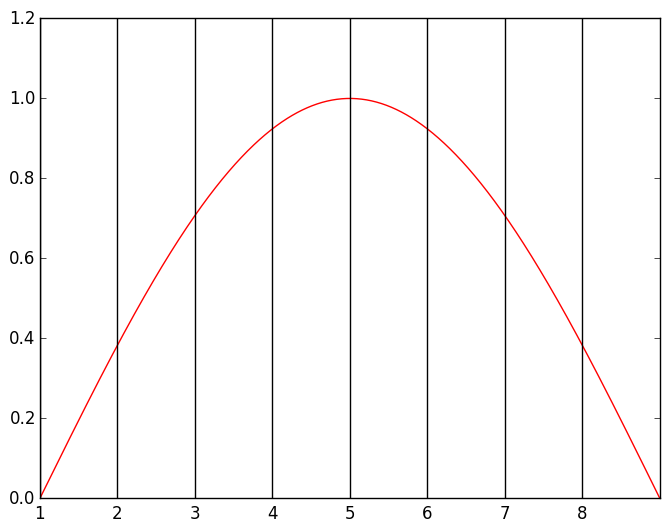
\includegraphics[width=7.5cm]{images/singlebasis_2}
      \vspace{-12px}
      \caption{7 grid points $i \in \{1..7\}$}
    \end{figure}
  \end{block}
\end{frame}

\begin{frame}
  \frametitle{Full Grid Discretization}
  \topline
  \vspace{-10px}
  \begin{block}{3. Basis function (standard hat function)}
    \begin{figure}[!htp]

      \setbeamertemplate{caption}{\raggedright\insertcaption\par}
      \setbeamerfont{caption}{size=\footnotesize}
      \centering
      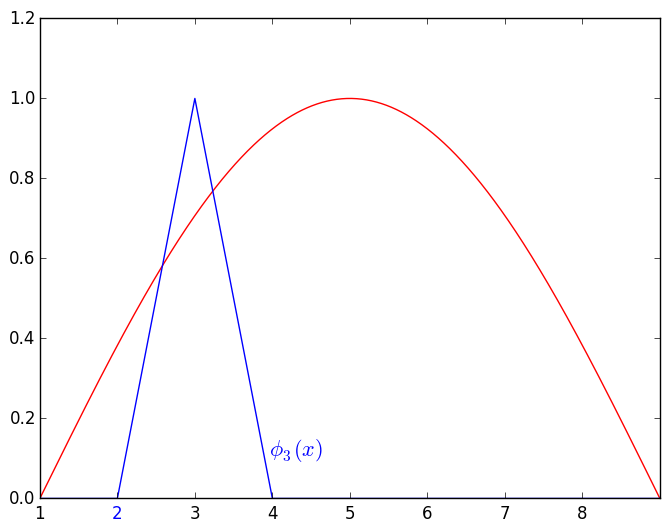
\includegraphics[width=7.5cm]{images/singlebasis_3}
      \vspace{-12px}
      \caption{$\phi(x - 3)$ with $\phi(x) = \text{max}(|1 - x|, 0)$}
    \end{figure}
  \end{block}
\end{frame}

\begin{frame}
  \frametitle{Full Grid Discretization}
  \topline
  \vspace{-10px}
  \begin{block}{4. Coefficient $\alpha$ (Surplus)}
    \begin{figure}[!htp]

      \setbeamertemplate{caption}{\raggedright\insertcaption\par}
      \setbeamerfont{caption}{size=\footnotesize}
      \centering
      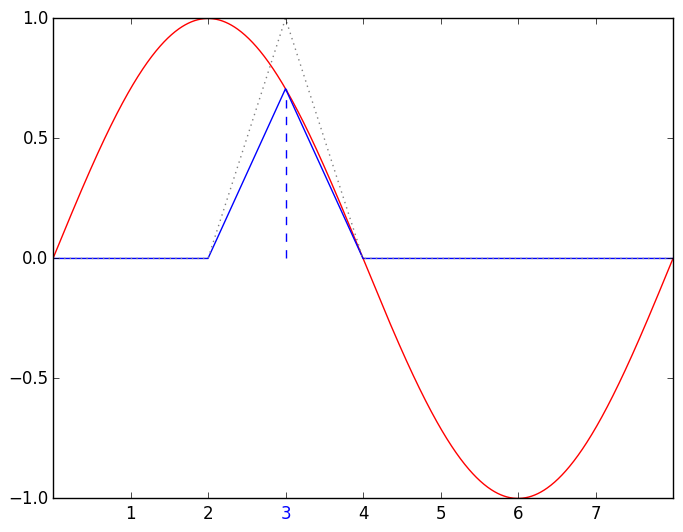
\includegraphics[width=7.5cm]{images/singlebasis_4}
      \vspace{-12px}
      \caption{$\alpha_3 \cdot \phi_3(x)$}
    \end{figure}
  \end{block}
\end{frame}

\begin{frame}
  \frametitle{Full Grid Discretization}
  \topline
  \vspace{-10px}
  \begin{block}{Sum over all basis functions}
    \begin{figure}[!htp]

      \setbeamertemplate{caption}{\raggedright\insertcaption\par}
      \setbeamerfont{caption}{size=\footnotesize}
      \centering
      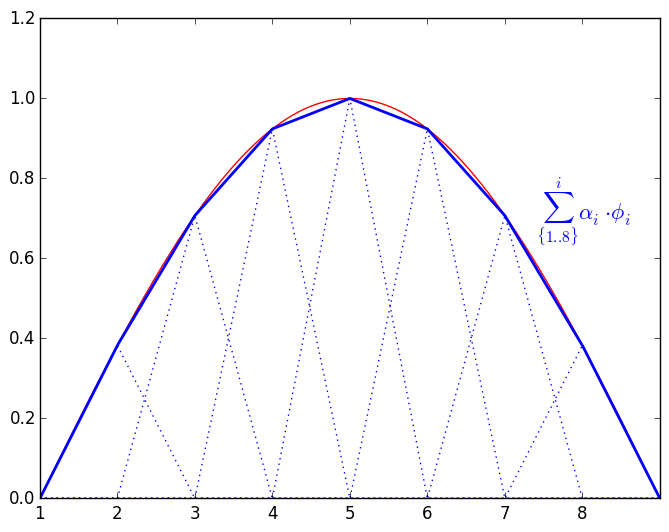
\includegraphics[width=7.5cm]{images/singlebasis_5}
      \vspace{-12px}
      \caption{$f(x) \approx \hat{f}(x) = \sum_i{\alpha_i \phi_i}$}
    \end{figure}
  \end{block}
\end{frame}

\begin{frame}
  \frametitle{Full Grid Discretization}
  \topline
  \vspace{-10px}
  \begin{block}{Sum over all basis functions}
    \begin{figure}[!htp]

      \setbeamertemplate{caption}{\raggedright\insertcaption\par}
      \setbeamerfont{caption}{size=\footnotesize}
      \centering
      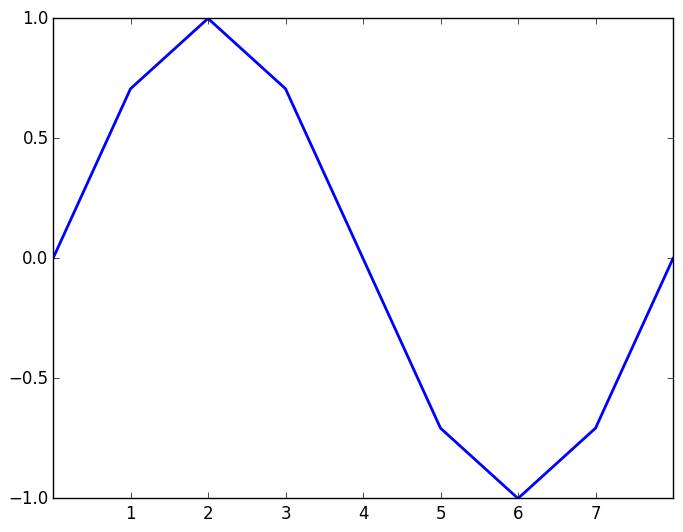
\includegraphics[width=7.5cm]{images/singlebasis_6}
      \vspace{-12px}
      \caption{$f(x) \approx \hat{f}(x) = \sum_i{\alpha_i \phi_i}$}
    \end{figure}
  \end{block}
\end{frame}

\begin{frame}
  \frametitle{Full Grid Discretization}
  \topline
  \vspace{-10px}
  \begin{block}{Full grid discretization in one dimension}
    \setbeamertemplate{enumerate items}[default]
    \begin{enumerate}
    \item A function $f(x)$ to discretize
    \item Grid points indexed by $i \in \{1,2,\dots\}$
    \item Basis functions; i.e. hat function $\phi(x)=\text{max}(1 - |x|, 0)$
    \item Coefficients $\alpha_i$ (Surpluses)
    \end{enumerate}
    \vspace{10px}
    \begin{center}
      $f(x) \approx$ $\hat{f}(x) = \sum_{i}^{}{\alpha_i \phi_i(x)}$
    \end{center}
  \end{block}
\end{frame}

\begin{frame}
  \frametitle{Full Grid Discretization}
  \topline
  \vspace{-10px}
  \begin{block}{$d > 1$ dimensions}
    \begin{itemize}
      \item Grid points as $d$--tuple, i.e. $(1,3,1)$
      \item Tensor product over one dimensional basis functions
    \end{itemize}
    \begin{center}
      $$ \phi_i(\vec{x}) = \prod_{j=1}^d{\phi_{i,j}(x_j)}$$
      $$ f(\vec{x}) \approx \hat{f}(\vec{x}) =
      \sum_i{\alpha_i\phi_i(\vec{x})}$$
    \end{center}
  \end{block}
\end{frame}

\begin{frame}
  \frametitle{Full Grid Discretization}
  \topline
  \vspace{-10px}
  \begin{block}{Full grid with $d = 2$}

    \begin{figure}[!htb]
      \setbeamertemplate{caption}{\raggedright\insertcaption\par}
      \setbeamerfont{caption}{size=\footnotesize}
      \minipage{0.5\textwidth}
      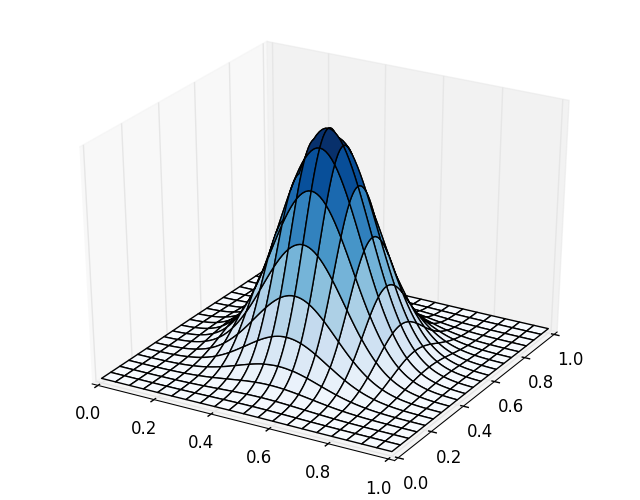
\includegraphics[width=\linewidth]{images/2dgrid_1_1.png}
      \vspace{-12px}
      \caption{$f(x) = \mathcal{N}(\vec{x})$}
      \endminipage
      \minipage{0.5\textwidth}
      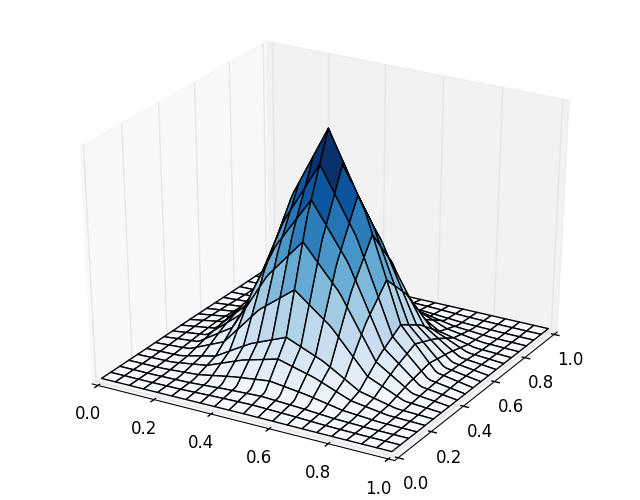
\includegraphics[width=\linewidth]{images/2dgrid_2_1.png}
      \vspace{-12px}
      \caption{Full grid discretization $\hat{f}(\vec{x})$}
      \endminipage
    \end{figure}
  \end{block}
\end{frame}

\begin{frame}
  \frametitle{Full Grid Discretization}
  \topline
  \vspace{-10px}
  \begin{block}{Full grid with $d = 2$}

    \begin{figure}[!htb]
      \setbeamertemplate{caption}{\raggedright\insertcaption\par}
      \setbeamerfont{caption}{size=\footnotesize}
      \minipage{0.5\textwidth}
      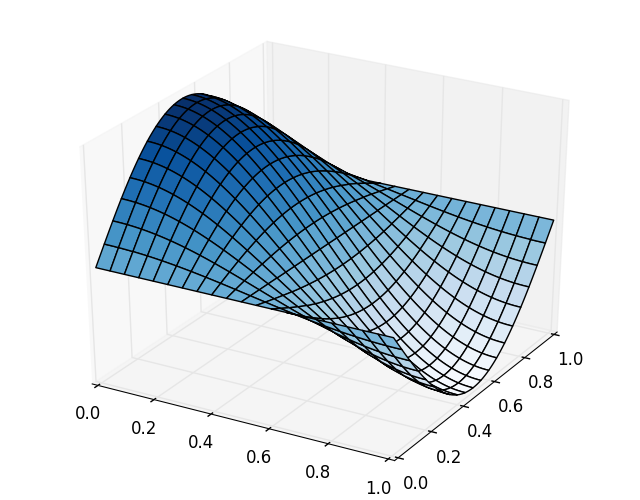
\includegraphics[width=\linewidth]{images/2dgrid_1_2.png}
      \vspace{-12px}
      \caption{$f(x) = \text{sin}(x_1) \cdot \text{cos}(x_2)$}
      \endminipage
      \minipage{0.5\textwidth}
      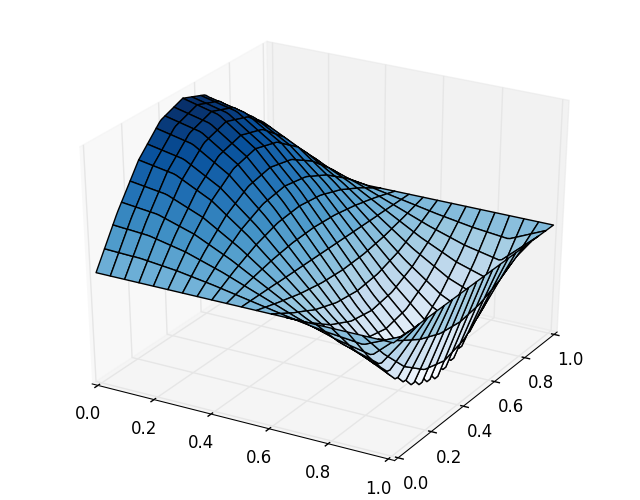
\includegraphics[width=\linewidth]{images/2dgrid_2_2.png}
      \vspace{-12px}
      \caption{Full grid discretization $\hat{f}(\vec{x})$}
      \endminipage
    \end{figure}
  \end{block}
\end{frame}

\begin{frame}
  \frametitle{Full Grid Discretization}
  \topline
  \vspace{-10px}
  \begin{block}{Summary}
    \begin{itemize}
      \item Grid points $i \in \{1,2,\dots,N\}^d$ defining $\phi_i(x)$
        \vspace{5px}
        \item For $d > 1$: \textbf{product} of 1D basis functions: \\
          $$\phi_i(\vec{x}) = \prod_{j=1}^d{\phi_{i,j}(x_j)}$$
        \item \textbf{Sum} over all weighted basis functions: \\
          $$\hat{f}(\vec{x}) = \sum_{i=1}^N{\alpha_i \phi_i(\vec{x})}$$
    \end{itemize}

  \end{block}
\end{frame}

%%% Local Variables:
%%% TeX-master: "slides"
%%% End:

\begin{frame}
  \frametitle{Sparse Grids -- Basics}
  \topline
  \vspace{-10px}
  \begin{block}{Hirachial Basis}
    \begin{figure}[!htp]
      \setbeamertemplate{caption}{\raggedright\insertcaption\par}
      \setbeamerfont{caption}{size=\footnotesize}
      \centering
      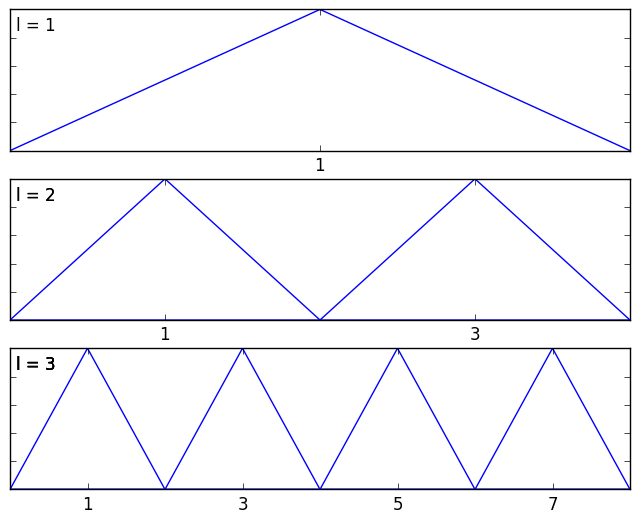
\includegraphics[width=7.5cm]{images/sparse_hats}
      \vspace{-12px}
      \caption{}
    \end{figure}
  \end{block}
\end{frame}

\begin{frame}
  \frametitle{Sparse Grids -- Basics}
  \topline
  \vspace{-10px}
  \begin{block}{Hirachial basis (vs nodal basis)}
    \begin{itemize}
      \item Grouping gridpoints into levels $l \in \{1,2,3\dots\}$
      \item Basis function by index \textbf{and} level: $\phi_{l,i}(x)$
    \end{itemize}
    \vspace{20px}
    \begin{center}
      $\hat{f}(x) = \sum_{l,i}{\ \alpha_{l,i} \cdot \phi_{l,i}(x)}$
    \end{center}
  \end{block}
\end{frame}

\begin{frame}
  \frametitle{Sparse Grids -- Basics}
  \topline
  \vspace{-10px}
  \begin{block}{Hirachial Basis}
    \begin{figure}[!htp]
      \setbeamertemplate{caption}{\raggedright\insertcaption\par}
      \setbeamerfont{caption}{size=\footnotesize}
      \centering
      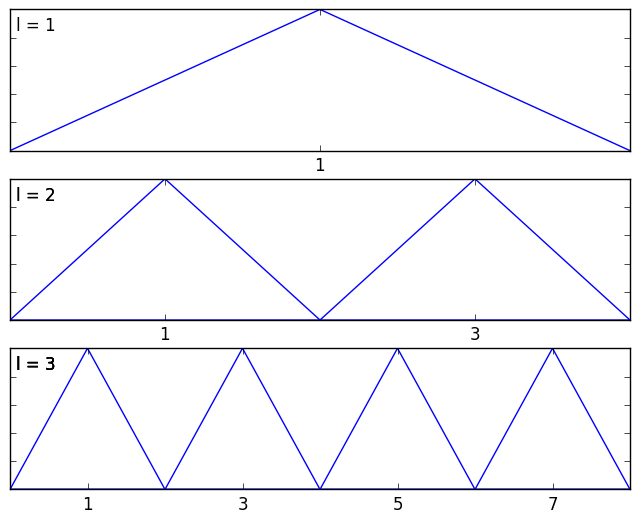
\includegraphics[width=7.5cm]{images/sparse_hats}
      \vspace{-12px}
      \caption{}
    \end{figure}
  \end{block}
\end{frame}

\begin{frame}
  \frametitle{Sparse Grids -- Basics}
  \topline
  \vspace{-10px}
  \begin{block}{Hirachial vs. nodal  basis}
    \begin{figure}[!htp]
      \setbeamertemplate{caption}{\raggedright\insertcaption\par}
      \setbeamerfont{caption}{size=\footnotesize}
      \centering
      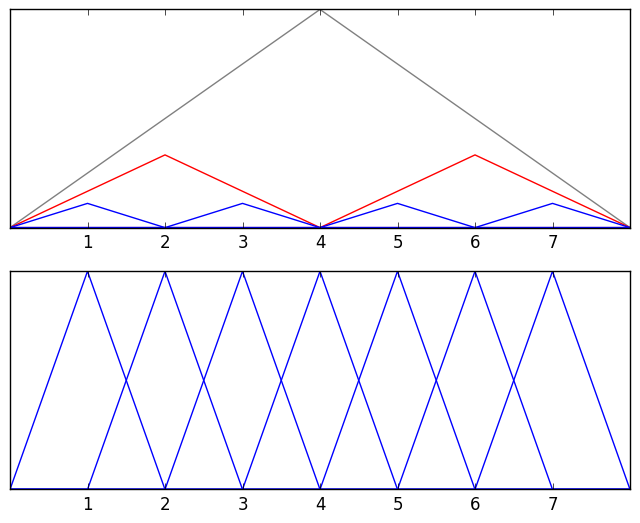
\includegraphics[width=7.5cm]{images/sparse_together}
      \vspace{-12px}
      \caption{}
    \end{figure}
  \end{block}
\end{frame}

\begin{frame}
  \frametitle{Sparse Grids -- Basics}
  \topline
  \vspace{-10px}
  \begin{block}{Full grid discretization: Hirachial basis}
    \begin{figure}[!htp]
      \setbeamertemplate{caption}{\raggedright\insertcaption\par}
      \setbeamerfont{caption}{size=\footnotesize}
      \centering
      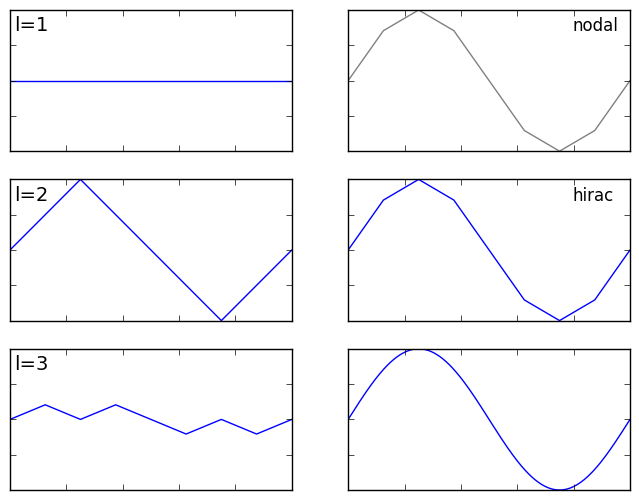
\includegraphics[width=7.5cm]{images/sparsegrid_1d}
      \vspace{-12px}
      \caption{}
    \end{figure}
  \end{block}
\end{frame}

\begin{frame}
  \frametitle{Sparse Grids -- Basics}
  \topline
  \vspace{-10px}
  \begin{block}{Basis function subspaces}
    \begin{itemize}
      \item Combination of levels through all dimensions
    \end{itemize}
  \end{block}
\end{frame}

\begin{frame}
  \frametitle{Sparse Grids -- Basics}
  \topline
  \vspace{-10px}
  \begin{block}{Hirachical gridpoints}
    \begin{figure}[!htp]
      \setbeamertemplate{caption}{\raggedright\insertcaption\par}
      \setbeamerfont{caption}{size=\footnotesize}
      \centering
      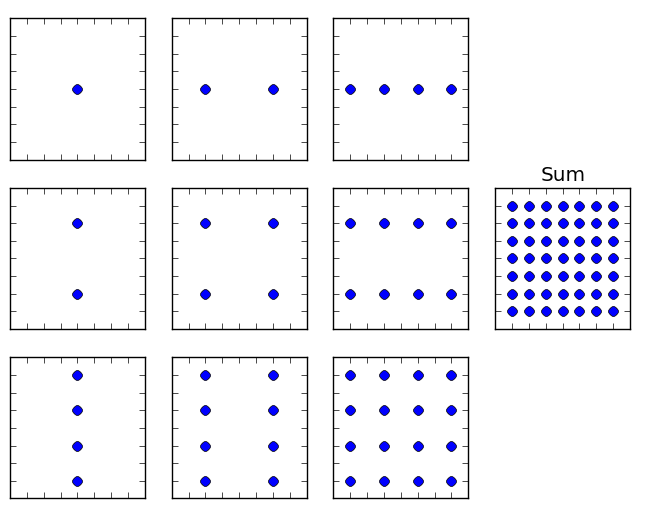
\includegraphics[width=7.5cm]{images/sparsegrid_hirach1}
      \vspace{-12px}
      \caption{}
    \end{figure}
  \end{block}
\end{frame}

\begin{frame}
  \frametitle{Sparse Grids -- Basics}
  \topline
  \vspace{-10px}
  \begin{block}{Hirachical subspaces}
    \begin{figure}[!htp]
      \setbeamertemplate{caption}{\raggedright\insertcaption\par}
      \setbeamerfont{caption}{size=\footnotesize}
      \centering
      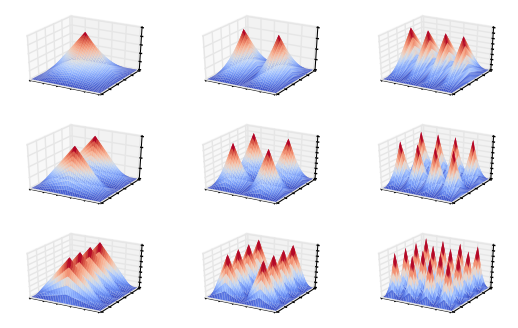
\includegraphics[width=7.5cm]{images/sparsegrid_2dhats}
      \vspace{-12px}
      \caption{}
    \end{figure}
  \end{block}
\end{frame}

\begin{frame}
  \frametitle{Sparse Grids -- Basics}
  \topline
  \vspace{-10px}
  \begin{block}{Sparse grid -- Changes}
    \begin{itemize}
      \item Throwing away certain subspaces
      \item Finding those is a \emph{a-priori} solvable optimization problem
      \item The resulting gird is now \textbf{sparse}
      \end{itemize}
  \end{block}
  \begin{block}{Profit}
    \begin{itemize}
      \item Reducing the computational effort ``a lot''
      \item Maintaining ``high'' accuracy
      \end{itemize}
  \end{block}
\end{frame}

\begin{frame}
  \frametitle{Sparse Grids -- Basics}
  \topline
  \vspace{-10px}
  \begin{block}{A \emph{sparse} grid}
    \begin{figure}[!htp]
      \setbeamertemplate{caption}{\raggedright\insertcaption\par}
      \setbeamerfont{caption}{size=\footnotesize}
      \centering
      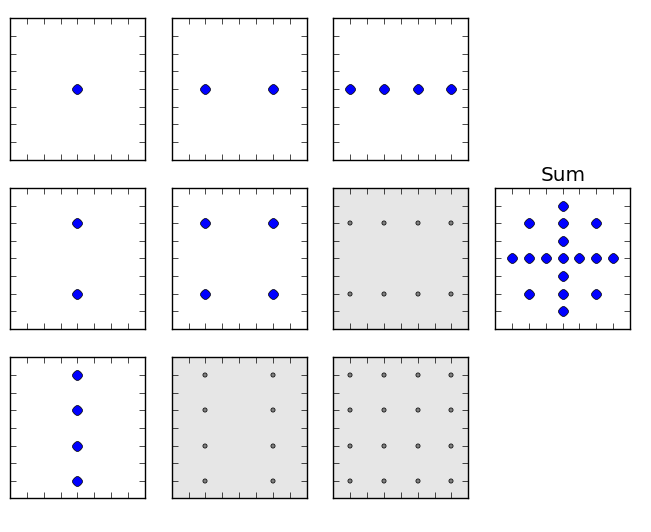
\includegraphics[width=7.5cm]{images/sparsegrid_hirach2}
      \vspace{-12px}
      \caption{}
    \end{figure}
  \end{block}
\end{frame}

\begin{frame}
  \frametitle{Sparse Grids -- Basics}
  \topline
  \vspace{-10px}
  \begin{block}{Boundry and smoothness}
    \begin{itemize}
      \item Boundries need special treatment
      \item The function needs to be sufficient smooth \\
        $D^2f$ needs to be bounded
      \end{itemize}
  \end{block}
  \begin{block}{Adaptivity}
    \begin{itemize}
      \item \emph{A-posteriori} modifications to better fit the function
      \item Picking a single gridpoint and adding level of detail around it
      \item Prone to overfitting and huge computational effort
      \end{itemize}
  \end{block}
\end{frame}


\begin{frame}
  \frametitle{Sparse Grids -- Basics}
  \topline
  \vspace{-10px}
  \begin{block}{Summary}
    \begin{itemize}
      \item Hirachial basis through grouping gridpoints into levels
      \item Creating ``subspaces'' through combination of levels in dimensions
      \item Selecting and combining subspaces
      \end{itemize}
  \end{block}
  \begin{block}{To keep in mind}
    \begin{itemize}
      \item Smoothness requirement for $f(x)$
      \item Boundry treatment
      \item Accuracy--effort trade-off
      \item Adaptivity options (\emph{a-posteriori})
      \end{itemize}
  \end{block}
\end{frame}



%%% Local Variables:
%%% TeX-master: "slides"
%%% End:


\end{document}